\chapter{Applying the Flow Equations}\label{Results}
\section{1D Bose Polaron in the Heavy Impurity Limit}
\subsection{Using the Flow Equation Appraoch}
\subsubsection{In combination with Bogoliubov-Transformation}
\begin{figure}[H]
    \centering
    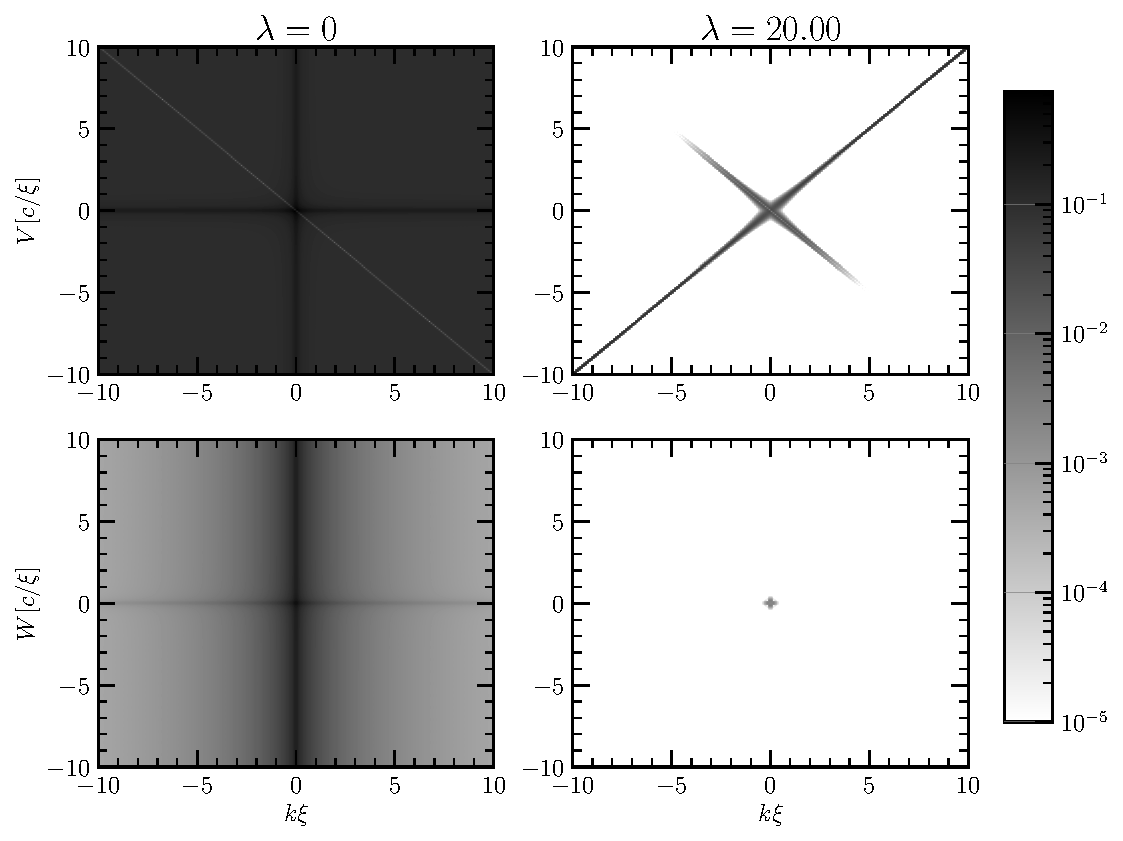
\includegraphics[width=\textwidth]{figures/plots/PDF/FlowIllustration.pdf}
    \caption[Flow Visualization for $\eta=10$]{Visualization of how the flow progresses for $\eta=10$ by shading larger absolute values for $V_{k,k^\prime},W_{k,k^\prime}$ darker. It is of note that on the ordinate and abscissa $0\widehat = \pm \lambda_{IR}\xi=\pm 0.1$. We see that good suppression occurs for all $W_{k,k^\prime}$, with slower convergence for smaller $|k|,|k^\prime|$.  Meanwhile, the matrix elements near the diagonal $V_{k,k}$ decay significantly slower than most off-diagonal elements. Also, matrix elements $V_{k,-k}$ converge, but to a value different from zero. Note that the values of $V$ near the main diagonal would  become even smaller if the flow were to progress further. This can be checked numerically by evaluating if $\mathrm{sgn}\left( V_{k,k^\prime}\right)=-\mathrm{sgn}\left( \partial_\lambda V_{k,k^\prime}\right)$ is fulfilled.}
    \label{FlowIllustration}
\end{figure}
As seen in Figure \ref{FlowIllustration}, the flow equations achieve the desired diagonalization except for terms $V_{k,-k}$. This is because $\omega_k=\omega_{-k}\forall k$ implies that the first order contribution in $\partial_\lambda V_{k,-k} =...$ vanishes. This is not a problem for the main diagonal terms $V_{k,k}$ because those have been "manually" set to zero by moving them in the diagonal part $\ham_0$ of the Hamiltonian. We can conclude that if we were not to stop the flow at a finite $\lambda$, our Hamiltonian would be approximately of the form 
\begin{equation}
\ham^\prime \defeq \Sum_{k}\left(\tilde\omega_k \CR_k\AN_k + \tilde V_{k,-k}\CR_k\AN_{-k}\right)
\end{equation}
for some $\tilde\omega_k,\tilde V_{k,k^\prime}$.\\
In principle, this could be brought into diagonal form by performing a Bogoliubov transformation for each summand by hand. But we will use the more general Bogoliubov transformation \ref{Bogoliubov Transformation Def} instead because, as can be seen in the figure \ref{FlowIllustrationInsufficient}, there are interaction strengths where not all $W_{k,k^\prime}$ vanish.
\begin{figure}[H]
    \centering
    \includegraphics[width=\textwidth]{figures/plots/PDF/FlowIllustration\_insufficient\_convergence.pdf}
    \caption[Flow Visualization for $\eta=-5.1$]{Visualization of the flow progression for $\eta=-5.1$ analogous to Figure \ref{FlowIllustration}. We can see that for this $\eta$ not all of the $W_{k,k^\prime}$ vanish, which may be related to the fact that we are now observing a system with a thermodynamic instability, as will become clear later on. The entailing negative eigenenergies can lead to unexpected behavior of the second order terms in the flow equations.}
    \label{FlowIllustrationInsufficient}
\end{figure}
One might think that we are therefore at an inherently poor starting point for making predictions about interesting system properties such as the ground state energy. However, it turns out that the many matrix elements that are actually suppressed sufficiently quickly dominate the behavior for the ground state energy to such an extent that if one discards all off-diagonal elements (regardless of their magnitude) after a certain point in the flow, very good agreement with the ground state energy predicted by a Bogoliubov transformation can be obtained.
\begin{figure}[H]
    \centering
    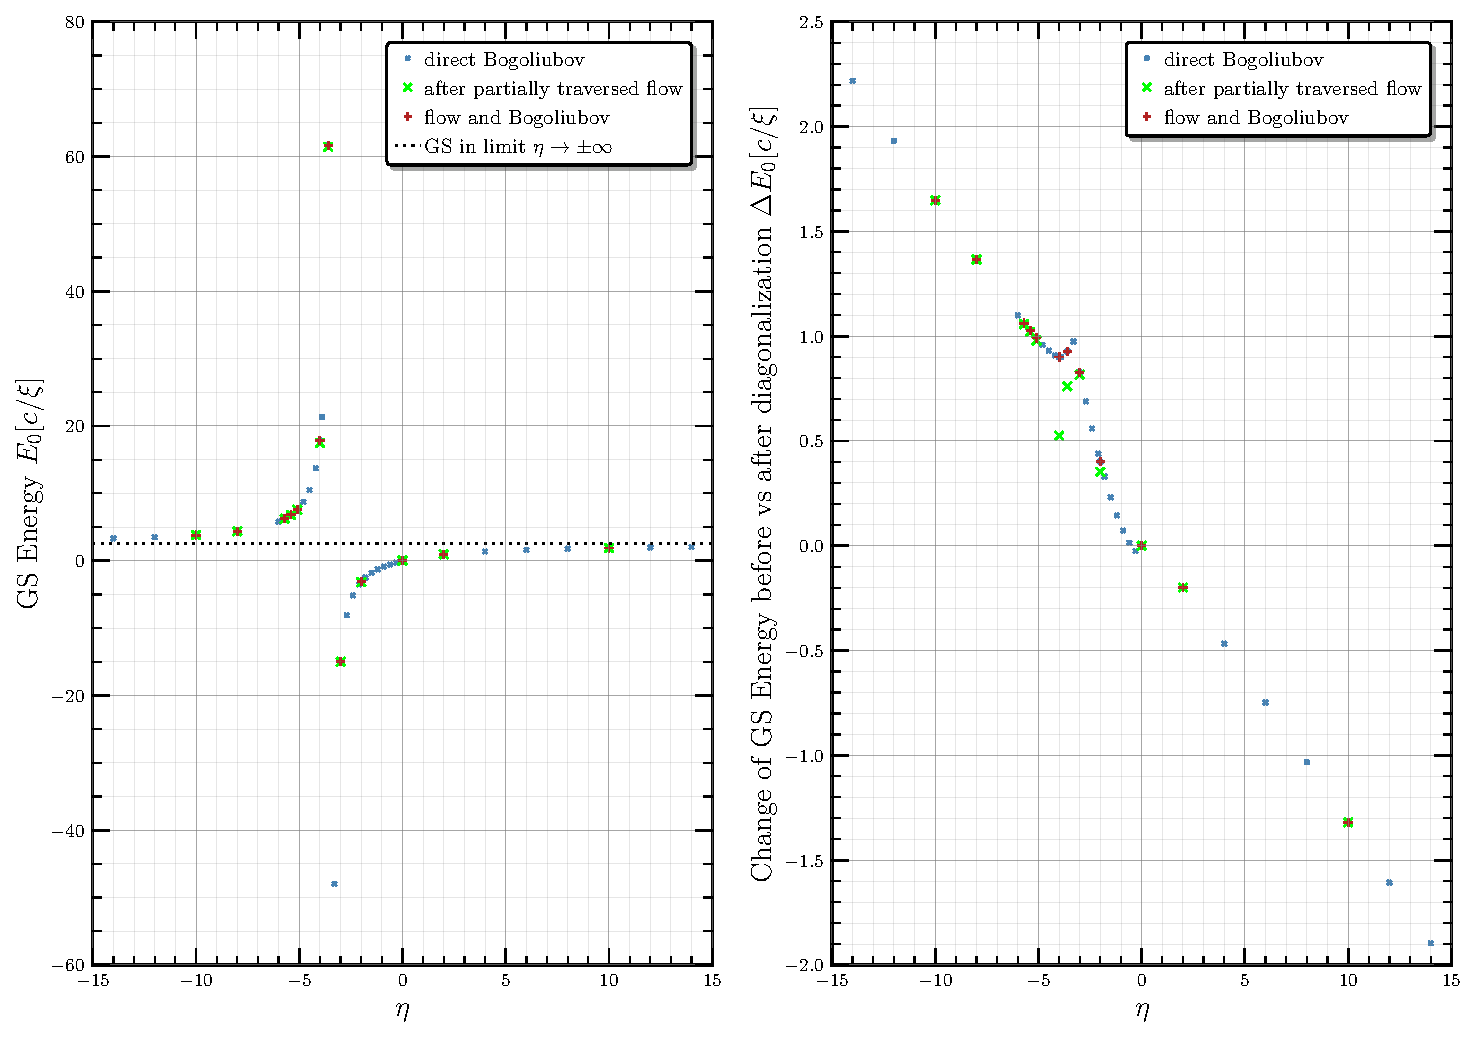
\includegraphics[width=\textwidth]{figures/plots/PDF/GS_energies_bog_flow_comp.pdf}
    \caption[Ground state energy of Bose Polaron for different $\eta$]{The left subplot shows the ground state energy for different $\eta$. The results are obtained via three different approaches: First a Bogoliubov transformation\footnote{For the numerics we again refer to the source code "Bogoliubov\_Transformation.py" in \url{https://github.com/SufficientlySmooth/Bachelor-Thesis-Numerics}} is applied directly to the Hamiltonian \ref{Ham_LLP_qudratic}. Second, the ground state energy is given by the constant $\epsilon$ in the flow Hamiltonian \ref{Flow_Hamiltonian_for_purely_quadratic_case} if all off-diagonal elements are neglected after a sufficiently long traversal of the flow. Third, the off-diagonal elements are not neglected but instead set to zero by a Bogoliubov Transformation of the flow Hamiltonian after traversing the flow for as long as in the second case.
The right subplot shows the difference between the ground state energy and the constant terms in the Hamiltonian \ref{Ham_LLP_qudratic} to highlight the (slight) differences between the three approaches.\\
It is noteworthy that the ground state energy in the limit $\eta\rightarrow\pm\infty$ is the same. This is because the two branches are expected to be adiabatically connected\cite{Grusdt_2017}. 
}
    \label{GSenergiesBogFlow}
\end{figure}
The agreement of the first and third approach in Figure \ref{GSenergiesBogFlow} is not surprising, since the flow equation approach transforms the Hamiltonian in infinitesimal \emph{unitary} steps. The surprisingly good behavior of the second method seems plausible when we consider that $\mathcal O(N^2)$ flows towards the diagonal, where of course the unitarity of the transformation conserves the trace of Hamiltonian (i.e. the sum of its eigenenergies). The number of $V_{k,k^\prime}$ that do not converge to 0 is only $\mathcal O(N)$, and the number of $W_{k,k^\prime}$ that do not converge to 0 is $\mathcal O(1)$. Therefore, assuming that these terms converge to values that are too large and do not diverge, we expect negligible contributions of these terms to the sum of the eigenenergies if a unitary transformation were performed that would actually make these terms vanish. Now, because the ground state energy depends on the sum of the eigenvalues \cite{PracticalTraining}, the prediction for the ground state energy for our system is very accurate. But this does not necessarily mean that all eigenenergies that are predicted by the flow equations are accurate. 
\begin{figure}[H]
    \centering
    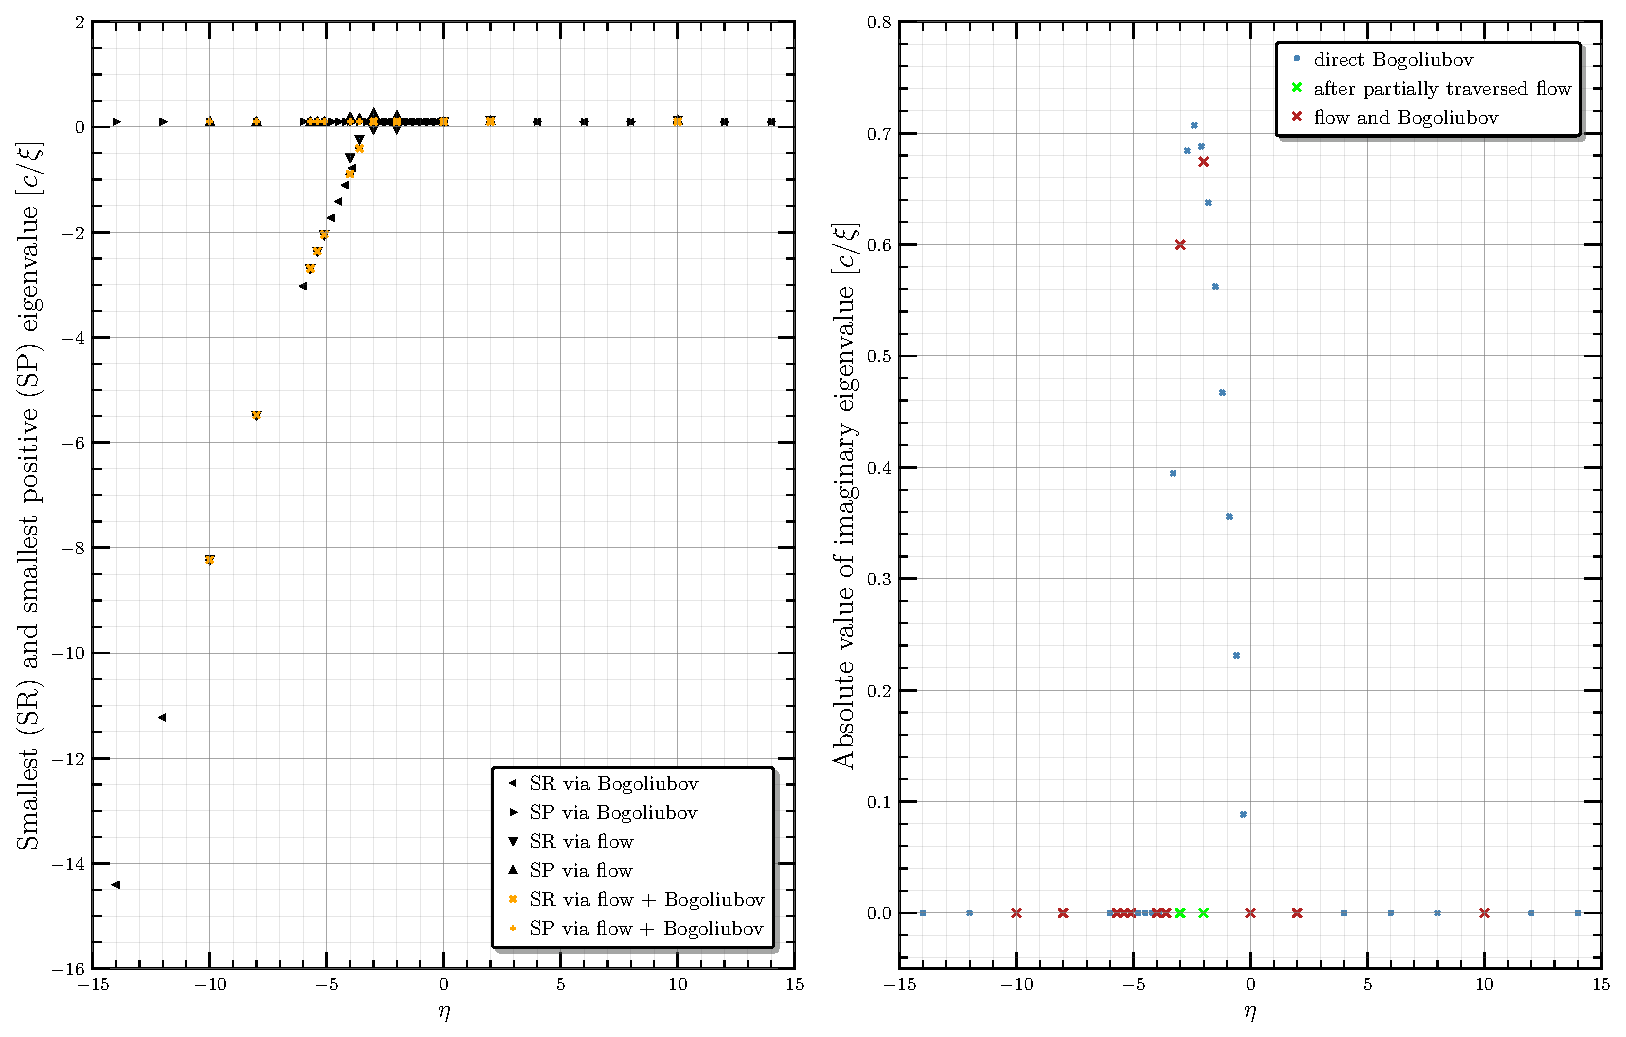
\includegraphics[width=\textwidth]{figures/plots/PDF/spectrum_analysis_bog_flow_comp.pdf}
    \caption[Characteristic eigenenergies of the Bose Polaron for different $\eta$]{The left subplot shows the smallest real (SR) and smallest real positive (SP) eigenvalues of the Hamiltonian for different $\eta$. The right subplot illustrates for which regimes dynamical instabilities (i.e. imaginary eigenvalues) occur.
}
    \label{SpectrumAnalysis}
\end{figure}
For example, the difference in the ground state energy in Figure \ref{GSenergiesBogFlow} for $\eta\approx -3.5$, which becomes especially clear when looking at the right subplot, can be explained by the fact that in this regime imaginary eigenvalues are to be expected (see Figure \ref{SpectrumAnalysis}). The flow equations cannot "see" these eigenvalues because the original Hamiltonian is real and the flow equations are algebraically closed in the sense that the flow cannot generate terms from $\C\setminus \R$ if it starts with purely real terms. If the flow equation approach is applied to a Hamiltonian with complex eigenenergies, those will be encoded in behaviour as seen in Figure \ref{FlowIllustrationInsufficient} where not all off-diagonal terms vanish. \\
The thermodynamic instability region for $-3.5\gtrsim\eta$, on the other hand, is correctly predicted in accordance with the results obtained by a Bogoliubov Transformation.
%The transformation \ref{twisted_trafo} then follows by again discretizing the momentum space. 
\subsubsection{Convergence improvement using twisted boundary conditions}
We will now try to improve the convergence properties of the off-diagonal matrix elements using the transformation
\begin{equation} \label{twisted_trafo}
\left\{\Delta k_n\right\}_{n\in\Z}\rightarrow \left\{\Delta k_n+\frac{\varphi}{L}\right\}_{n\in\Z}
\end{equation}
 which (slightly) shifts the grid of $k$-values and thereby breaks the symmetry $k\leftrightarrow -k$ by introducing a phase parameter $\varphi\in\R$. Notice that in the limit $\phi\rightarrow 0$ we recover the original, symmetrical grid. \\
This transformation is not merely a mathematically convenient trick but is also physically meaningful. If we consider our BEC in which the impurity is immersed arranged in circular form we expect periodic boundary conditions
\begin{equation}
\psi(x)=\psi(x+L)
\end{equation}
on a wave function $\psi$ describing some part of the system. However, introducing a magnetic flux $\theta$ in the ring imposes \emph{twisted} periodic boundary conditions:
\begin{equation}
\psi(x)=e^{i\varphi}\psi(x+L)
\end{equation}
It can then be shown \cite{twisted} that these twisted boundary conditions are equivalent to the shift 
\begin{equation}
-i\partial_x\rightarrow -i\partial x+\frac{\varphi}{L}
\end{equation}
or, after recognizing the momentum operator in position representation, 
\begin{equation}
k\rightarrow k+\frac{\varphi}{L}.
\end{equation}
%\subsection{Using a Bogoliubov Transformation}
\section{Comparison of the two Approaches}
